\documentclass[10pt,a4paper]{article}
\usepackage{ctex}
\usepackage{fancyhdr}
\usepackage{booktabs}
\usepackage{graphicx}
\usepackage{amsmath}
\usepackage{float}
\usepackage{xcolor}
\usepackage{listings}
\usepackage{multirow}
\usepackage{diagbox}
\usepackage[table]{xcolor}
\usepackage[colorlinks,linkcolor=blue]{hyperref} % 用于插入超链接

% 文章页面margin设置
\usepackage[a4paper]{geometry}
\geometry{top=1in}
\geometry{bottom=1in}
\geometry{left=0.75in}
\geometry{right=0.75in}   % 设置上下左右页边距
\geometry{marginparwidth=1.75cm}    % 设置边注距离(注释、标记等)

% 设置页眉
\pagestyle{fancy}
\fancyhf{}
\lhead{汇编语言第一次大作业}
\chead{小组成员:袁晨圃、王荦璠、曾子恒、王永生}
\rhead{\thepage}
\renewcommand{\headrulewidth}{0.4pt}

% 代码设置
\lstset{
    basicstyle=\ttfamily\small,
    numbers=left,
    numberstyle=\tiny,
    keywordstyle=\color{blue},
    commentstyle=\color{green!60!black},
    stringstyle=\color{red},
    breaklines=true,
    frame=single,
    showstringspaces=false
}

\begin{document}

\begin{center}
    \LARGE{\textbf{汇编语言第一次大作业实验报告}}
    
    \vspace{0.5cm}
    \large{小组成员:袁晨圃、王荦璠、曾子恒、王永生}
    
    \vspace{0.3cm}
    \today
\end{center}

\section{实验总体思路及过程}

\begin{itemize}
    \item \textbf{总体思路}:采用字典树(Trie树)对输入内容进行处理,找到出现次数最多的单词并输出
    \item \textbf{数据结构设计}:
    \begin{itemize}
        \item 使用字典树存储单词,每个节点表示一个字符
        \item 使用数组实现树结构,避免指针操作的复杂性
        \item 全局数据存储在variable.s中,主要包括以下数组:
        \begin{lstlisting}[language=C]
son[MAXN][CHARSET_SIZE]  // 存储当前节点的子节点,son[i][ch]表示节点i的字符ch子节点的ID
cnt[MAXN]                // 记录每个单词出现的次数
father[MAXN]             // 记录每个节点的父节点ID,用于回溯
content[MAXN]            // 存储每个节点对应的字符
max_id[MAXN]             // 存储出现次数最多的单词的节点ID
        \end{lstlisting}
        
        \item 关键常量定义:
        \begin{lstlisting}[language=C]
#define MAXN         2500  // 字典树的最大节点数
#define MAXL         100   // 单词的最大长度
#define CHARSET_SIZE 128   // 字符集大小(ASCII)
        \end{lstlisting}
    \end{itemize}
    \item \textbf{实验过程}:
    \begin{itemize}
        \item 为分工合作,首先使用组员们熟悉的C语言实现了对输入内容的处理,将代码分为4大功能模块,分别是:
        
        \begin{lstlisting}[language=C]
int main();     // 读入输入,调用子模块
void alpha();   // 处理字母,构建字典树
void not_alpha(); // 处理非字母,分割单词
void output(int id); // 从叶子节点回溯到根节点,输出单词
        \end{lstlisting}
        
        \item 处理流程:
        \begin{enumerate}
            \item 逐个读取输入字符
            \item 若是字母,则调用alpha()将其加入当前单词
            \item 若不是字母,则调用not\_alpha()处理当前单词结束
            \item 所有输入处理完毕后,输出出现次数最多的单词
        \end{enumerate}
        
        \item 4位小组成员每人负责将一个模块的代码用汇编语言实现,最后整合运行
        \item 小组成员的协作通过github进行代码共享,本次实验还通过makefile部署了自动化开发流程,自动对各模块进行编译,测试和合并运行
    \end{itemize}
\end{itemize}

\section{实验分工}

\begin{itemize}
    \item \textbf{袁晨圃}:main.s函数编写,代码整合测试
    \item \textbf{王荦璠}:alpha.s函数编写,实验报告撰写
    \item \textbf{曾子恒}:not\_alpha.s函数编写,实验报告撰写
    \item \textbf{王永生}:output.s函数编写,实验报告撰写
\end{itemize}

\section{汇编程序设计方法}

\subsection{总体设计思路}

\begin{itemize}
    \item \textbf{模块化分层设计}:通过不同的函数模块实现不同的功能,清晰划分责任
    \item \textbf{数据逻辑分离}:利用variable.s文件集中管理全局数据结构,其他文件通过.extern引用
    \item \textbf{数据结构选择}:
    \begin{itemize}
        \item 采用字典树(Trie树)实现单词存储和频率统计,时间复杂度、空间复杂度均为 \(O(n)\),其中 \(n\) 为文本长度
        \item 使用线性数组实现树结构,避免复杂的指针操作
        \item variable.s中定义的核心数据结构:
        \begin{lstlisting}[language={[x86masm]Assembler}]
.section .data
son:     .fill MAXN*CHARSET_SIZE, 4, 0  # int son[MAXN][CHARSET_SIZE] = {0}
cnt:     .fill MAXN, 4, 0               # int cnt[MAXN] = {0}
father:  .fill MAXN, 4, 0               # int father[MAXN] = {0}
max_id:  .fill MAXN, 4, 0               # int max_id[MAXN] = {0}
content: .fill MAXN, 1, 0               # char content[MAXN] = {0}
tot:     .long 0                        # int tot = 0
max_cnt: .long 0                        # int max_cnt = 0
max_siz: .long 0                        # int max_siz = 0
ch:      .long 0                        # int ch = 0
cur_id:  .long 0                        # int cur_id = 0
        \end{lstlisting}
    \end{itemize}
    \item \textbf{编程风格}:
    \begin{itemize}
        \item 使用位置无关代码(PIC)技术访问全局变量
        \item 充分利用64位寄存器和地址计算指令
        \item 严格遵循函数调用约定(保存被调用者保存寄存器)
        \item 合理利用C标准库函数,如 \verb|getchar()|、\verb|puts()| 等
    \end{itemize}
\end{itemize}

\subsection{分模块具体设计}

\subsubsection{main.s}

\begin{enumerate}
    \item \textbf{主程序设计}
    \begin{itemize}
        \item 使用外部符号声明,引入需要用到的函数和全局变量:
        \begin{lstlisting}[language={[x86masm]Assembler}]
.globl _start
.extern isalpha, alpha, not_alpha, output, debug, fflush
.extern ch, max_id, max_siz
        \end{lstlisting}
    \end{itemize}
    
    \item \textbf{主循环处理输入}
    \begin{itemize}
        \item \textbf{循环读取字符}:调用 \verb|getchar| 读取输入,遇 \verb|EOF| 结束循环
        \begin{lstlisting}[language={[x86masm]Assembler}]
.while_cond:
    call    getchar
    movl    %eax, ch(%rip) # let ch = getchar()
    cmpl    $-1, %eax
    je      .while_end      # jump ch == EOF ? while_end : if_cond
        \end{lstlisting}
        
        \item \textbf{字符分类处理}:
        \begin{itemize}
            \item \textbf{判断是否为字母}:
            \begin{lstlisting}[language={[x86masm]Assembler}]
.if_cond:
    movl    ch(%rip), %edi
    call    isalpha
    testl   %eax, %eax
    jz      .else_stmt      # jump isalpha(ch) ? if_stmt : else_stmt
            \end{lstlisting}
            
            \item \textbf{字母}:调用 \verb|alpha| 处理字母字符,构建单词
            \item \textbf{非字母}:调用 \verb|not_alpha| 处理非字母字符,用于分割单词
        \end{itemize}
    \end{itemize}
    
    \item \textbf{结果输出阶段}
    \begin{itemize}
        \item \textbf{遍历高频词数组}:按 \verb|max_siz| 遍历 \verb|max_id| 数组,调用 \verb|output| 逐项输出高频词
        \begin{lstlisting}[language={[x86masm]Assembler}]
    movq    $0, %rsi # let counter %rsi = 0
.for_loop:
    cmpl    max_siz(%rip), %esi
    jge     .for_end # if %esi >= max_siz then break
    leaq    max_id(%rip), %rdi # let %rdi = &max_id
    movl    (%rdi,%rsi,4), %edi # let %edi = max_id[%esi]
    movslq  %edi, %rdi # sign extend %edi to %rdi
    push    %rsi        # 保存循环计数器
    call    output      # call output(max_id[%esi])
    pop     %rsi        # 恢复循环计数器
    inc     %rsi        # %esi++
    jmp     .for_loop
        \end{lstlisting}
    \end{itemize}
    
    \item \textbf{收尾与调试}
    \begin{itemize}
        \item \textbf{调试}:调用 \verb|debug| 打印内部数据结构(如树节点)
        \item \textbf{刷新输出}:\verb|fflush(NULL)| 强制写入流,确保缓冲区内容被输出
        \begin{lstlisting}[language={[x86masm]Assembler}]
    xor     %edi, %edi
    call    fflush       # call fflush(NULL)
        \end{lstlisting}
        \item \textbf{退出程序}:使用syscall直接调用系统退出
        \begin{lstlisting}[language={[x86masm]Assembler}]
    movl    $60, %eax    # syscall number for exit
    xorl    %edi, %edi   # exit code 0
    syscall
        \end{lstlisting}
    \end{itemize}
\end{enumerate}

\subsubsection{alpha.s}

\begin{enumerate}
    \item \textbf{函数入口准备}
    \begin{itemize}
        \item \textbf{栈帧建立}:\verb|pushq %rbp| + \verb|movq %rsp, %rbp| 创建新栈帧
        \item \textbf{外部依赖}:通过 \verb|.extern| 声明使用外部全局变量(树结构核心数据)
    \end{itemize}
    
    \item \textbf{子节点地址计算}
    \begin{lstlisting}[language={[x86masm]Assembler}]
movl  cur_id(%rip), %eax      # 当前节点ID
movl  ch(%rip), %ecx          # 输入字符ASCII值
imull $CHARSET_SIZE, %eax     # 计算二维数组行偏移(CHARSET_SIZE=128)
addl  %ecx, %eax              # 列偏移叠加(cur_id*128 + ch)
leaq  son(%rip), %rdx         # 获取son数组基址
leaq  (%rdx,%rax,4), %rsi     # 最终地址:&son[cur_id][ch]
    \end{lstlisting}
    \begin{itemize}
        \item 核心目的是定位 \verb|son[cur_id][ch]| 在内存中的地址
    \end{itemize}
    
    \item \textbf{子节点存在性检查}
    \begin{lstlisting}[language={[x86masm]Assembler}]
cmpl  $0, (%rsi)              # 检查子节点是否存在
jne   .skip_creation          # 存在则跳过创建
    \end{lstlisting}
    \begin{itemize}
        \item 作用:判断当前字符是否已存在子节点路径
    \end{itemize}
    
    \item \textbf{新节点创建逻辑}
    \begin{itemize}
        \item 计数器递增:\verb|incl tot| 全局唯一ID生成
        \item 父节点记录:\verb|father[tot] = cur_id| 记录新节点的父节点
        \item 字符存储:\verb|content[tot] = ch| 存储当前字符到新节点
        \item 子节点注册:\verb|son[cur_id][ch] = tot| 绑定父子关系
    \end{itemize}
    
    \item \textbf{当前节点更新}
    \begin{lstlisting}[language={[x86masm]Assembler}]
movl  (%rsi), %eax            # 获取子节点ID(新建或已有)
movl  %eax, cur_id(%rip)      # 更新cur_id为子节点
    \end{lstlisting}
    \begin{itemize}
        \item 状态转移:将当前节点指针移动到子节点,准备处理下一字符
    \end{itemize}
    
    \item \textbf{函数返回}
    \begin{itemize}
        \item 栈帧恢复:\verb|leave| + \verb|ret| 恢复调用前环境
    \end{itemize}
\end{enumerate}

\subsubsection{not\_alpha.s}

\begin{enumerate}
    \item \textbf{栈帧与寄存器保护}(行1-4)
    \begin{itemize}
        \item 建立栈帧并保存 rbx/r12/r13 寄存器,遵循 x64 调用约定
        \item 使用 PIC(位置无关代码)模式访问全局变量,通过 @GOTPCREL(\%rip) 实现
    \end{itemize}
    
    \item \textbf{有效性检查}(行5-9)
    \begin{itemize}
        \item 检查 \verb |cur_id| 是否为 0(空状态)
        \item 若为 0 直接跳转到退出流程,避免无效节点操作
    \end{itemize}
    
    \item \textbf{词频统计}(行10-14)
    \begin{itemize}
        \item 从 \verb|cnt| 数组中读取 \verb |cur_id| 对应的词频值
        \item 将词频值加 1 后写回内存,完成计数器更新
    \end{itemize}
    
    \item \textbf{最大词频更新}(行15-22)
    \begin{itemize}
        \item 分支1(新最大值):
        \begin{itemize}
            \item 若当前词频超过 \verb|max_cnt|,更新 \verb|max_cnt| 为新值
            \item 清空 \verb|max_siz|(重置极值数组索引)
        \end{itemize}
        \item 分支2(等于当前最大值):
        \begin{itemize}
            \item 将 \verb|cur_id| 写入 \verb|max_id| 数组末尾
            \item 递增 \verb|max_siz| 记录新的极值数量
        \end{itemize}
    \end{itemize}
    
    \item \textbf{状态重置}(行23-25)
    \begin{itemize}
        \item 将 \verb|cur_id| 重置为 0,准备接收下一个单词的插入操作
    \end{itemize}
    
    \item \textbf{退出清理}(行26-29)
    \begin{itemize}
        \item 恢复保存的寄存器
        \item 销毁栈帧并返回调用点
    \end{itemize}
\end{enumerate}

\subsubsection{output.s}

\begin{enumerate}
    \item \textbf{函数基本结构与内存布局}
    \begin{itemize}
        \item 输出缓冲区定义及常量声明:
        \begin{lstlisting}[language={[x86masm]Assembler}]
.equ    MAXL, 1000

.section .bss
        .lcomm  output_buffer, MAXL*2

# 全局符号,由C文件提供
        .extern content                 # char  content[]
        .extern father                  # int   father[]
        .extern puts
        \end{lstlisting}
        \item 函数签名定义:
        \begin{lstlisting}[language={[x86masm]Assembler}]
.section .text
        .globl  output
        .type   output, @function

#  void output(int id)
#  %edi 为参数 id
        \end{lstlisting}
    \end{itemize}
    
    \item \textbf{栈帧与寄存器保护}
    \begin{itemize}
        \item 建立栈帧并保存 \verb|%rbx|(被调用者保存寄存器),分配16字节局部空间
        \item 初始化局部变量 cnt=0(记录字符收集数量)
        \begin{lstlisting}[language={[x86masm]Assembler}]
        pushq   %rbp
        movq    %rsp, %rbp
        pushq   %rbx                    # callee-saved

        subq    $16, %rsp               # 局部变量留 16 字节
        movl    $0, -4(%rbp)            # int cnt = 0;
        \end{lstlisting}
    \end{itemize}
    
    \item \textbf{字符反向收集}
    \begin{itemize}
        \item 循环条件:当 \verb|id| \(\neq 0\) 时持续遍历(\verb|father| 数组实现树结构回溯)
        \item 操作流程:
        \begin{lstlisting}[language={[x86masm]Assembler}]
.Lcollect:
        testl   %edi, %edi
        je      .Lreverse

        movl    -4(%rbp), %eax          # eax→rax = cnt(零扩展)
        lea     content(%rip), %rbx
        movzbl  (%rbx,%rdi,1), %ecx     # cl = content[id]

        lea     output_buffer(%rip), %rbx
        movb    %cl, (%rbx,%rax,1)      # output[cnt] = cl

        incl    -4(%rbp)                # ++cnt

        lea     father(%rip), %rbx
        movl    (%rbx,%rdi,4), %edi     # id = father[id]
        jmp     .Lcollect
        \end{lstlisting}
        \item 特性:收集的字符顺序为从叶子到根的反序(例如树中路径为 3→2→1,收集顺序为 [3], [2], [1]),需要后续反转
    \end{itemize}
    
    \item \textbf{字符串反转}
    \begin{itemize}
        \item 指针初始化:
        \begin{itemize}
            \item rsi 指向最后一个字符(output\_buffer + cnt-1)
            \item rdi 指向结束符位置(output\_buffer + cnt)
        \end{itemize}
        \item 反转过程:通过双指针从两端向中间交换字符,最终得到正序字符串
        \begin{lstlisting}[language={[x86masm]Assembler}]
.Lreverse:
        movl    -4(%rbp), %eax          # eax→rax = cnt
        movl    %eax, %edx              # edx→rdx = cnt
        decl    %eax                    # eax→rax = cnt-1

        lea     output_buffer(%rip), %rbx
        leaq    (%rbx,%rax,1), %rsi     # rsi = &output[cnt-1]
        leaq    (%rbx,%rdx,1), %rdi     # rdi = &output[cnt]
        movq    %rbx, %rcx              # rcx = &output[0]

.Lrev_loop:
        cmpq    %rcx, %rsi
        jb      .Lafter_reverse
        movzbl  (%rsi), %eax
        movb    %al, (%rdi)
        decq    %rsi
        incq    %rdi
        jmp     .Lrev_loop
        \end{lstlisting}
    \end{itemize}
    
    \item \textbf{终止符与输出}
    \begin{itemize}
        \item 安全设计:在 \verb|output_buffer[cnt*2]| 写入 \verb|\0|(确保缓冲区溢出时仍能终止)
        \item 栈对齐优化:调用 \verb|puts| 前调整栈指针保证16字节对齐
        \item 输出地址:将反转后的字符串起始地址(\verb|output_buffer + cnt|)传给 \verb|puts|
        \begin{lstlisting}[language={[x86masm]Assembler}]
.Lafter_reverse:
        movl    -4(%rbp), %eax
        sall    $1, %eax                # cnt * 2
        lea     output_buffer(%rip), %rbx
        movb    $0, (%rbx,%rax,1)       # '\0'

        /* ---------- 调用 puts ---------- */
        movl    -4(%rbp), %eax
        lea     output_buffer(%rip), %rdi
        leaq    (%rdi,%rax,1), %rdi     # rdi = 输出字符串地址

        subq    $8, %rsp                # 对齐栈 -> 16B
        call    puts@PLT
        addq    $8, %rsp

        popq    %rbx
        leave
        ret
        \end{lstlisting}
    \end{itemize}
\end{enumerate}

\section{编程调试心得体会}

\begin{itemize}
    \item C语言的代码在对单模块的调试中发挥了重要作用。通过 \verb|make debug-(模块名)| 命令可以将C语言编写的该模块替换为相应的汇编.s文件,在其他函数仍是C语言的情况下进行测试,实现单模块的调试。这是一种效率较高的debug方式。
    
    \item 各个成员在代码编写时都遇到了"位数"的问题,实验目标是实现64位的程序,makefile的编译指令中也是64位的编译指令。但各组员编写的时候都写成了32位程序,导致测试的时候出现错误。因此,在编写汇编代码时,需要注意指令的位数,以及数据类型是否正确。
    
    \item 在程序调试过程中,我们遇到了一个特别有趣的问题:程序执行正常,但没有任何输出显示在终端上。经过调试发现,程序的逻辑是正确的,但输出内容似乎"消失"了。经过仔细分析main.s的代码,我们发现问题出在程序的退出方式上:

    \begin{lstlisting}[language={[x86masm]Assembler}]
    movl    $60, %eax    # syscall number for exit
    xorl    %edi, %edi   # exit code 0
    syscall
    \end{lstlisting}

    这段代码使用了直接的系统调用来终止程序,而没有通过C运行时库的 \verb|exit()| 函数。问题在于,直接使用syscall退出程序会绕过C运行时的清理过程,导致标准输出流的缓冲区没有被刷新,输出内容仍然滞留在缓冲区中。

    我们通过两种方法解决了这个问题:
    \begin{enumerate}
        \item 在syscall之前调用 \verb|fflush(NULL)| 手动刷新所有输出缓冲区
        \item 替换直接系统调用,改为调用C库的 \verb|exit()| 函数,让它来处理程序终止时的缓冲区刷新
    \end{enumerate}

    这个经验让我们深刻理解了汇编代码与C运行时环境之间的交互,特别是关于输出缓冲机制和程序正确终止的重要性。
\end{itemize}

\section{源代码及测试文件}

本项目的github仓库地址为:\url{https://github.com/ucas-asm2025-team/assignment1},其中包含了所有的源代码和测试文件。

\section{运行测试结果截图}

\begin{figure}[H]
	
	\begin{minipage}{0.49\linewidth}%可修改0.49为其他比例,调整大小
		\vspace{3pt}
		\centerline{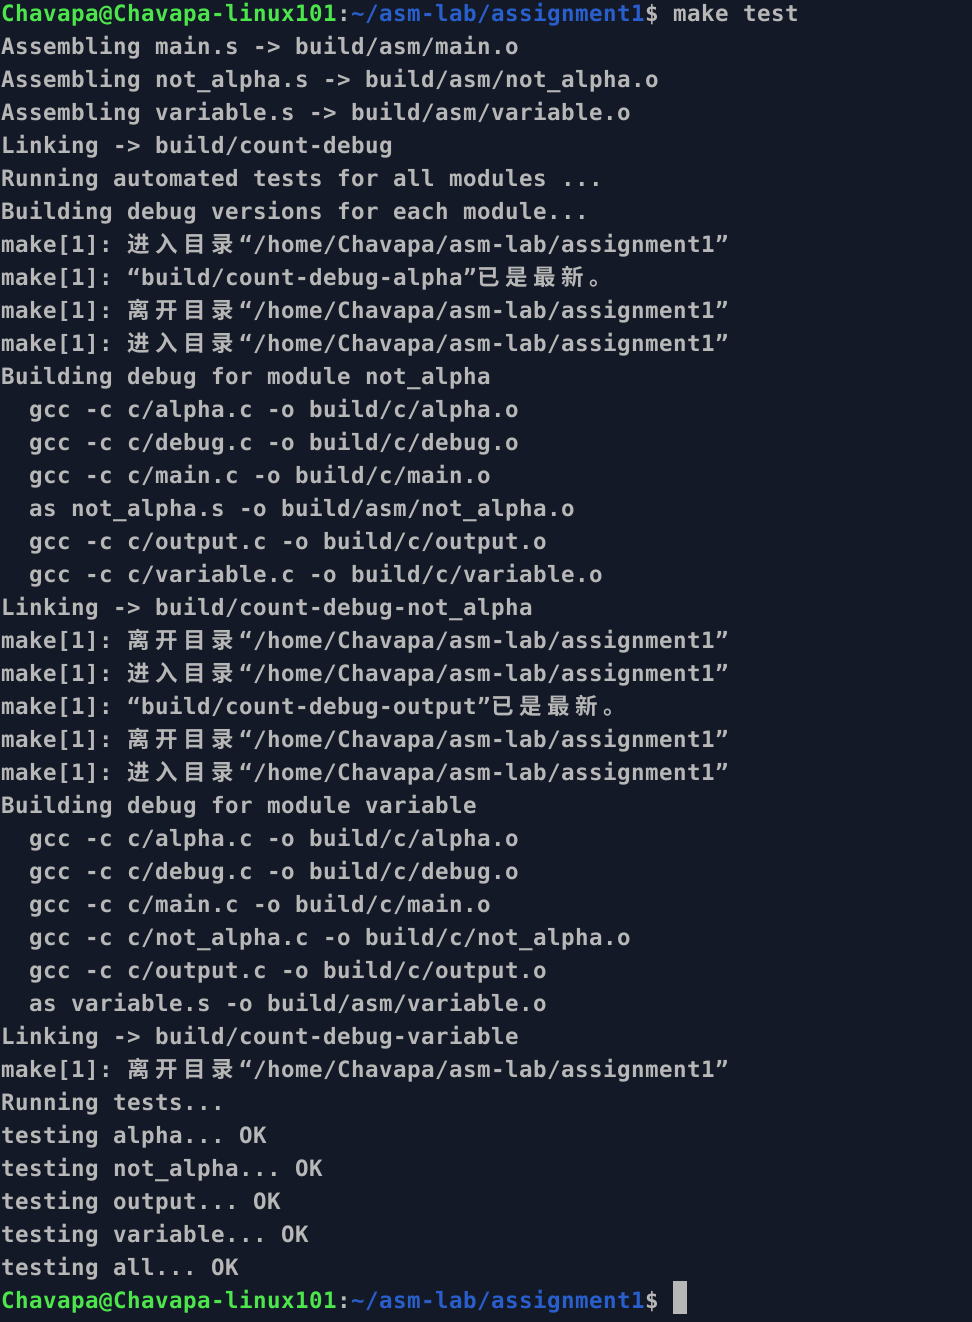
\includegraphics[width=\textwidth]{images/terminal_test.png}}
	\end{minipage}
	\begin{minipage}{0.49\linewidth}
		\vspace{3pt}
		\centerline{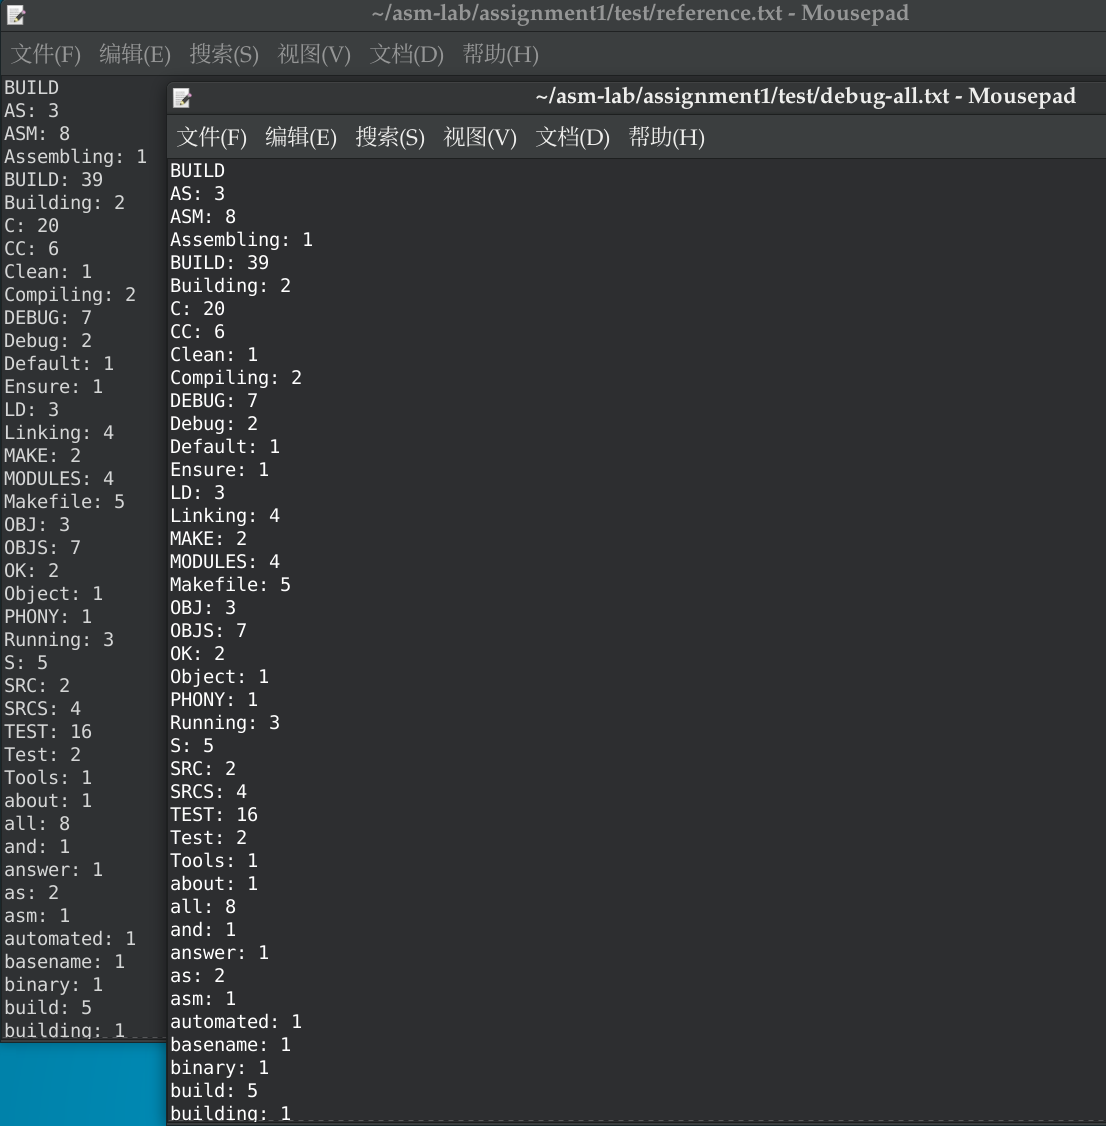
\includegraphics[width=\textwidth]{images/comparison.png}}
	\end{minipage}
 
	\caption{运行测试结果截图(左:终端测试;右:输出结果比对)}
\end{figure}

\end{document}
